

\begin{figure}[H]
 \centering
	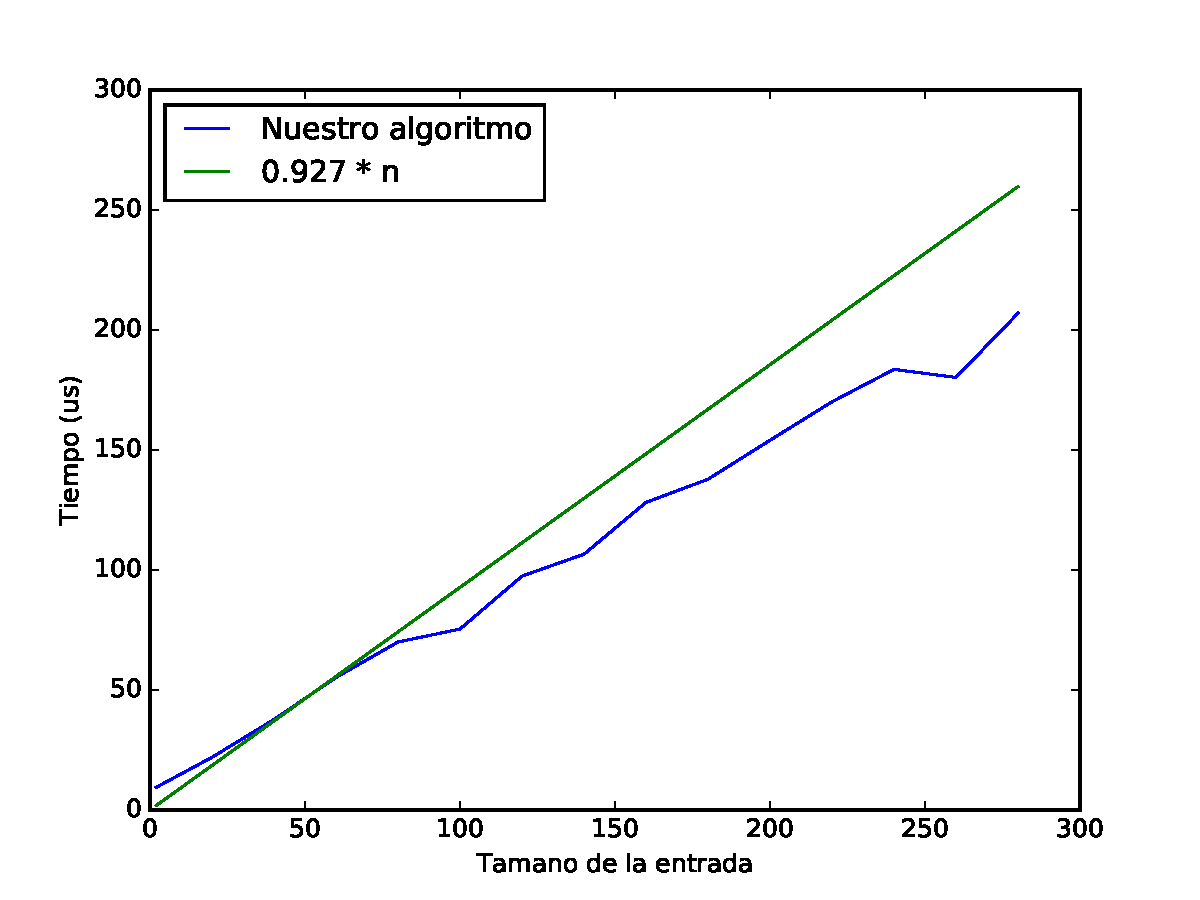
\includegraphics[width=0.8\textwidth]{img/exp/problema1-mejor.pdf}
	\caption{\footnotesize Tiempo que toma el algoritmo en $\mu$s para una entrada de tamaño $n$ ($m \in O(n))$.}
	\label{fig:problema1-mejor}
\end{figure}


\begin{figure}[H]
 \centering
	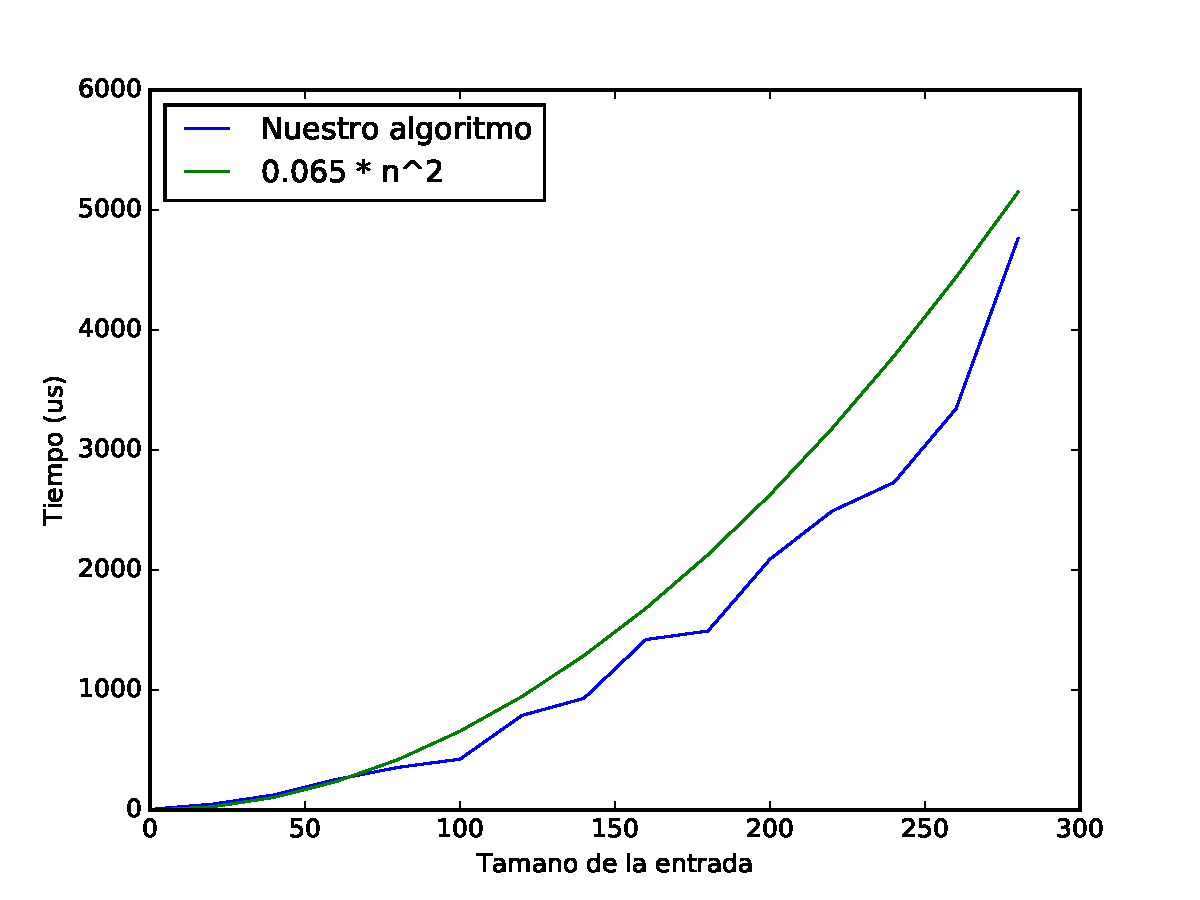
\includegraphics[width=0.8\textwidth]{img/exp/problema1-peor.pdf}
	\caption{\footnotesize Tiempo que toma el algoritmo en $\mu$s para una entrada de tamaño $n$ ($m \in O(n^2))$.}
	\label{fig:problema1-peor}
\end{figure}

\begin{figure}[H]
 \centering
	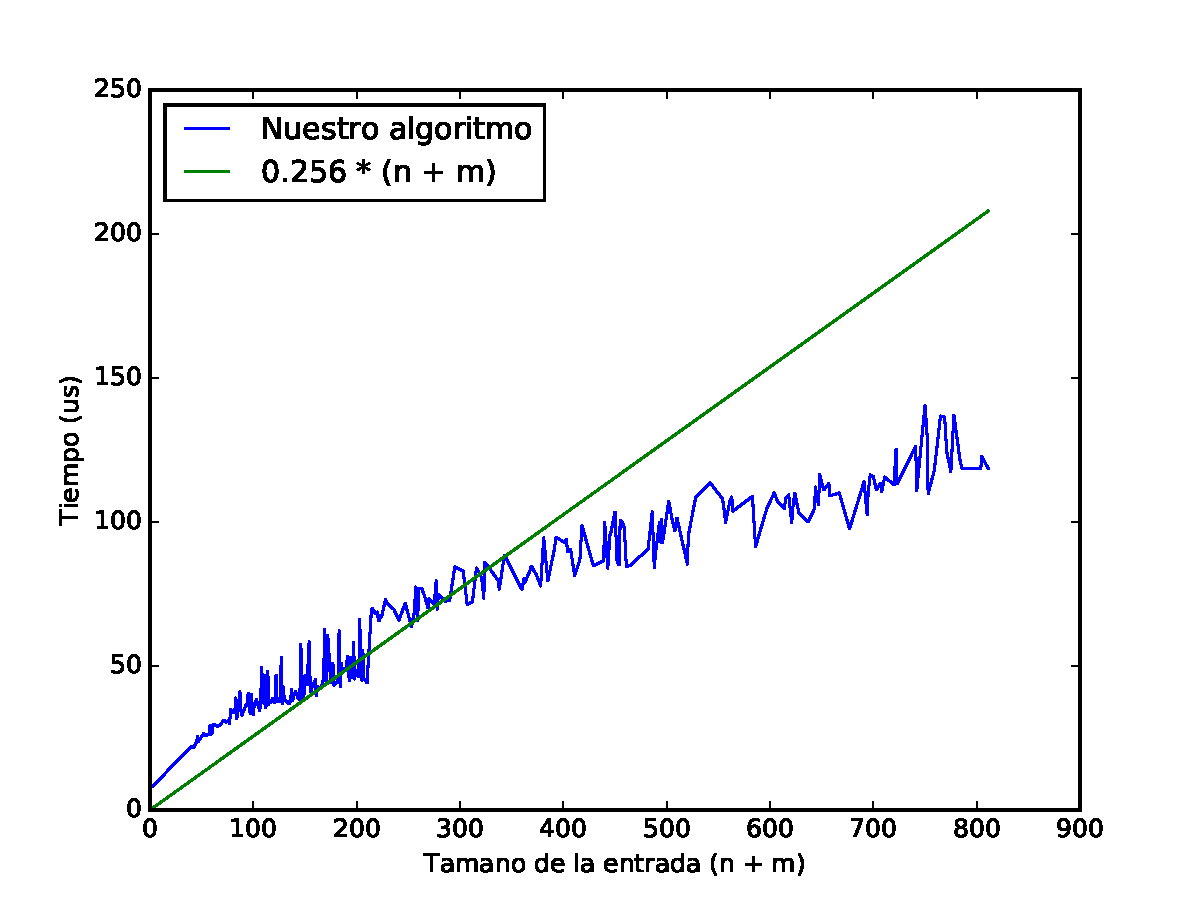
\includegraphics[width=0.8\textwidth]{img/exp/problema1-promedio.pdf}
	\caption{\footnotesize Tiempo que toma el algoritmo en $\mu$s para una entrada de tamaño $n + m$. $m$ al azar entre $n-1$ y $\frac{n(n-1)}{2}$.}
	\label{fig:problema1-promedio}
\end{figure}

\begin{figure}[H]
 \centering
	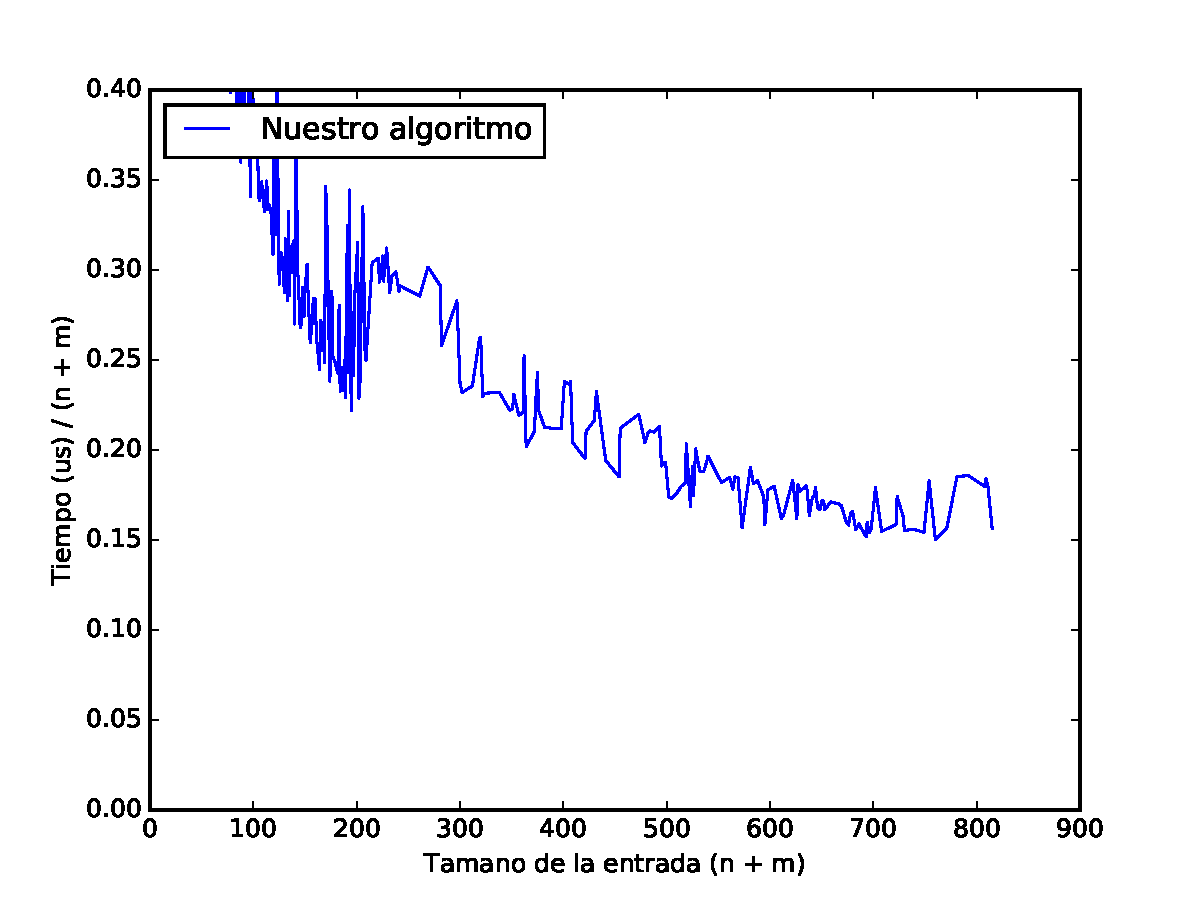
\includegraphics[width=0.8\textwidth]{img/exp/problema1-promedio2.pdf}
	\caption{\footnotesize Tiempo que toma el algoritmo en $\mu$s dividido $n + m$ para una entrada de tamaño $n + m$.  $m$ al azar entre $n-1$ y $\frac{n(n-1)}{2}$}
	\label{fig:problema1-promedio2}
\end{figure}

\subsubsection{M\'etodo de experimentación}
